% Options for packages loaded elsewhere
\PassOptionsToPackage{unicode}{hyperref}
\PassOptionsToPackage{hyphens}{url}
%
\documentclass[
]{article}
\usepackage{amsmath,amssymb}
\usepackage{iftex}
\ifPDFTeX
  \usepackage[T1]{fontenc}
  \usepackage[utf8]{inputenc}
  \usepackage{textcomp} % provide euro and other symbols
\else % if luatex or xetex
  \usepackage{unicode-math} % this also loads fontspec
  \defaultfontfeatures{Scale=MatchLowercase}
  \defaultfontfeatures[\rmfamily]{Ligatures=TeX,Scale=1}
\fi
\usepackage{lmodern}
\ifPDFTeX\else
  % xetex/luatex font selection
\fi
% Use upquote if available, for straight quotes in verbatim environments
\IfFileExists{upquote.sty}{\usepackage{upquote}}{}
\IfFileExists{microtype.sty}{% use microtype if available
  \usepackage[]{microtype}
  \UseMicrotypeSet[protrusion]{basicmath} % disable protrusion for tt fonts
}{}
\makeatletter
\@ifundefined{KOMAClassName}{% if non-KOMA class
  \IfFileExists{parskip.sty}{%
    \usepackage{parskip}
  }{% else
    \setlength{\parindent}{0pt}
    \setlength{\parskip}{6pt plus 2pt minus 1pt}}
}{% if KOMA class
  \KOMAoptions{parskip=half}}
\makeatother
\usepackage{xcolor}
\usepackage[margin=1in]{geometry}
\usepackage{color}
\usepackage{fancyvrb}
\newcommand{\VerbBar}{|}
\newcommand{\VERB}{\Verb[commandchars=\\\{\}]}
\DefineVerbatimEnvironment{Highlighting}{Verbatim}{commandchars=\\\{\}}
% Add ',fontsize=\small' for more characters per line
\usepackage{framed}
\definecolor{shadecolor}{RGB}{248,248,248}
\newenvironment{Shaded}{\begin{snugshade}}{\end{snugshade}}
\newcommand{\AlertTok}[1]{\textcolor[rgb]{0.94,0.16,0.16}{#1}}
\newcommand{\AnnotationTok}[1]{\textcolor[rgb]{0.56,0.35,0.01}{\textbf{\textit{#1}}}}
\newcommand{\AttributeTok}[1]{\textcolor[rgb]{0.13,0.29,0.53}{#1}}
\newcommand{\BaseNTok}[1]{\textcolor[rgb]{0.00,0.00,0.81}{#1}}
\newcommand{\BuiltInTok}[1]{#1}
\newcommand{\CharTok}[1]{\textcolor[rgb]{0.31,0.60,0.02}{#1}}
\newcommand{\CommentTok}[1]{\textcolor[rgb]{0.56,0.35,0.01}{\textit{#1}}}
\newcommand{\CommentVarTok}[1]{\textcolor[rgb]{0.56,0.35,0.01}{\textbf{\textit{#1}}}}
\newcommand{\ConstantTok}[1]{\textcolor[rgb]{0.56,0.35,0.01}{#1}}
\newcommand{\ControlFlowTok}[1]{\textcolor[rgb]{0.13,0.29,0.53}{\textbf{#1}}}
\newcommand{\DataTypeTok}[1]{\textcolor[rgb]{0.13,0.29,0.53}{#1}}
\newcommand{\DecValTok}[1]{\textcolor[rgb]{0.00,0.00,0.81}{#1}}
\newcommand{\DocumentationTok}[1]{\textcolor[rgb]{0.56,0.35,0.01}{\textbf{\textit{#1}}}}
\newcommand{\ErrorTok}[1]{\textcolor[rgb]{0.64,0.00,0.00}{\textbf{#1}}}
\newcommand{\ExtensionTok}[1]{#1}
\newcommand{\FloatTok}[1]{\textcolor[rgb]{0.00,0.00,0.81}{#1}}
\newcommand{\FunctionTok}[1]{\textcolor[rgb]{0.13,0.29,0.53}{\textbf{#1}}}
\newcommand{\ImportTok}[1]{#1}
\newcommand{\InformationTok}[1]{\textcolor[rgb]{0.56,0.35,0.01}{\textbf{\textit{#1}}}}
\newcommand{\KeywordTok}[1]{\textcolor[rgb]{0.13,0.29,0.53}{\textbf{#1}}}
\newcommand{\NormalTok}[1]{#1}
\newcommand{\OperatorTok}[1]{\textcolor[rgb]{0.81,0.36,0.00}{\textbf{#1}}}
\newcommand{\OtherTok}[1]{\textcolor[rgb]{0.56,0.35,0.01}{#1}}
\newcommand{\PreprocessorTok}[1]{\textcolor[rgb]{0.56,0.35,0.01}{\textit{#1}}}
\newcommand{\RegionMarkerTok}[1]{#1}
\newcommand{\SpecialCharTok}[1]{\textcolor[rgb]{0.81,0.36,0.00}{\textbf{#1}}}
\newcommand{\SpecialStringTok}[1]{\textcolor[rgb]{0.31,0.60,0.02}{#1}}
\newcommand{\StringTok}[1]{\textcolor[rgb]{0.31,0.60,0.02}{#1}}
\newcommand{\VariableTok}[1]{\textcolor[rgb]{0.00,0.00,0.00}{#1}}
\newcommand{\VerbatimStringTok}[1]{\textcolor[rgb]{0.31,0.60,0.02}{#1}}
\newcommand{\WarningTok}[1]{\textcolor[rgb]{0.56,0.35,0.01}{\textbf{\textit{#1}}}}
\usepackage{graphicx}
\makeatletter
\def\maxwidth{\ifdim\Gin@nat@width>\linewidth\linewidth\else\Gin@nat@width\fi}
\def\maxheight{\ifdim\Gin@nat@height>\textheight\textheight\else\Gin@nat@height\fi}
\makeatother
% Scale images if necessary, so that they will not overflow the page
% margins by default, and it is still possible to overwrite the defaults
% using explicit options in \includegraphics[width, height, ...]{}
\setkeys{Gin}{width=\maxwidth,height=\maxheight,keepaspectratio}
% Set default figure placement to htbp
\makeatletter
\def\fps@figure{htbp}
\makeatother
\setlength{\emergencystretch}{3em} % prevent overfull lines
\providecommand{\tightlist}{%
  \setlength{\itemsep}{0pt}\setlength{\parskip}{0pt}}
\setcounter{secnumdepth}{-\maxdimen} % remove section numbering
\ifLuaTeX
  \usepackage{selnolig}  % disable illegal ligatures
\fi
\usepackage{bookmark}
\IfFileExists{xurl.sty}{\usepackage{xurl}}{} % add URL line breaks if available
\urlstyle{same}
\hypersetup{
  pdftitle={Bioinformatics Assignment 2},
  hidelinks,
  pdfcreator={LaTeX via pandoc}}

\title{Bioinformatics Assignment 2}
\author{}
\date{\vspace{-2.5em}}

\begin{document}
\maketitle

\begin{Shaded}
\begin{Highlighting}[]
\CommentTok{\# Define file paths}
\NormalTok{data\_dir }\OtherTok{\textless{}{-}} \FunctionTok{file.path}\NormalTok{(}\StringTok{"../../data"}\NormalTok{, }\StringTok{"SRP164913"}\NormalTok{)}
\NormalTok{data\_file }\OtherTok{\textless{}{-}} \FunctionTok{file.path}\NormalTok{(data\_dir, }\StringTok{"SRP164913\_HUGO.tsv"}\NormalTok{)}
\NormalTok{metadata\_file }\OtherTok{\textless{}{-}} \FunctionTok{file.path}\NormalTok{(data\_dir, }\StringTok{"metadata\_SRP164913.tsv"}\NormalTok{)}
\NormalTok{results\_dir }\OtherTok{\textless{}{-}} \FunctionTok{file.path}\NormalTok{(}\StringTok{"../../results"}\NormalTok{)}
\NormalTok{plots\_dir }\OtherTok{\textless{}{-}} \FunctionTok{file.path}\NormalTok{(}\StringTok{"plots"}\NormalTok{)}

\CommentTok{\# Libraries}
\FunctionTok{library}\NormalTok{(DESeq2)}
\end{Highlighting}
\end{Shaded}

\begin{verbatim}
## Loading required package: S4Vectors
\end{verbatim}

\begin{verbatim}
## Loading required package: stats4
\end{verbatim}

\begin{verbatim}
## Loading required package: BiocGenerics
\end{verbatim}

\begin{verbatim}
## 
## Attaching package: 'BiocGenerics'
\end{verbatim}

\begin{verbatim}
## The following objects are masked from 'package:stats':
## 
##     IQR, mad, sd, var, xtabs
\end{verbatim}

\begin{verbatim}
## The following objects are masked from 'package:base':
## 
##     anyDuplicated, aperm, append, as.data.frame, basename, cbind,
##     colnames, dirname, do.call, duplicated, eval, evalq, Filter, Find,
##     get, grep, grepl, intersect, is.unsorted, lapply, Map, mapply,
##     match, mget, order, paste, pmax, pmax.int, pmin, pmin.int,
##     Position, rank, rbind, Reduce, rownames, sapply, setdiff, table,
##     tapply, union, unique, unsplit, which.max, which.min
\end{verbatim}

\begin{verbatim}
## 
## Attaching package: 'S4Vectors'
\end{verbatim}

\begin{verbatim}
## The following object is masked from 'package:utils':
## 
##     findMatches
\end{verbatim}

\begin{verbatim}
## The following objects are masked from 'package:base':
## 
##     expand.grid, I, unname
\end{verbatim}

\begin{verbatim}
## Loading required package: IRanges
\end{verbatim}

\begin{verbatim}
## Loading required package: GenomicRanges
\end{verbatim}

\begin{verbatim}
## Loading required package: GenomeInfoDb
\end{verbatim}

\begin{verbatim}
## Loading required package: SummarizedExperiment
\end{verbatim}

\begin{verbatim}
## Loading required package: MatrixGenerics
\end{verbatim}

\begin{verbatim}
## Loading required package: matrixStats
\end{verbatim}

\begin{verbatim}
## 
## Attaching package: 'MatrixGenerics'
\end{verbatim}

\begin{verbatim}
## The following objects are masked from 'package:matrixStats':
## 
##     colAlls, colAnyNAs, colAnys, colAvgsPerRowSet, colCollapse,
##     colCounts, colCummaxs, colCummins, colCumprods, colCumsums,
##     colDiffs, colIQRDiffs, colIQRs, colLogSumExps, colMadDiffs,
##     colMads, colMaxs, colMeans2, colMedians, colMins, colOrderStats,
##     colProds, colQuantiles, colRanges, colRanks, colSdDiffs, colSds,
##     colSums2, colTabulates, colVarDiffs, colVars, colWeightedMads,
##     colWeightedMeans, colWeightedMedians, colWeightedSds,
##     colWeightedVars, rowAlls, rowAnyNAs, rowAnys, rowAvgsPerColSet,
##     rowCollapse, rowCounts, rowCummaxs, rowCummins, rowCumprods,
##     rowCumsums, rowDiffs, rowIQRDiffs, rowIQRs, rowLogSumExps,
##     rowMadDiffs, rowMads, rowMaxs, rowMeans2, rowMedians, rowMins,
##     rowOrderStats, rowProds, rowQuantiles, rowRanges, rowRanks,
##     rowSdDiffs, rowSds, rowSums2, rowTabulates, rowVarDiffs, rowVars,
##     rowWeightedMads, rowWeightedMeans, rowWeightedMedians,
##     rowWeightedSds, rowWeightedVars
\end{verbatim}

\begin{verbatim}
## Loading required package: Biobase
\end{verbatim}

\begin{verbatim}
## Welcome to Bioconductor
## 
##     Vignettes contain introductory material; view with
##     'browseVignettes()'. To cite Bioconductor, see
##     'citation("Biobase")', and for packages 'citation("pkgname")'.
\end{verbatim}

\begin{verbatim}
## 
## Attaching package: 'Biobase'
\end{verbatim}

\begin{verbatim}
## The following object is masked from 'package:MatrixGenerics':
## 
##     rowMedians
\end{verbatim}

\begin{verbatim}
## The following objects are masked from 'package:matrixStats':
## 
##     anyMissing, rowMedians
\end{verbatim}

\begin{Shaded}
\begin{Highlighting}[]
\FunctionTok{library}\NormalTok{(ggplot2)}
\FunctionTok{library}\NormalTok{(magrittr)}
\end{Highlighting}
\end{Shaded}

\begin{verbatim}
## 
## Attaching package: 'magrittr'
\end{verbatim}

\begin{verbatim}
## The following object is masked from 'package:GenomicRanges':
## 
##     subtract
\end{verbatim}

\begin{Shaded}
\begin{Highlighting}[]
\FunctionTok{library}\NormalTok{(M3C)}
\FunctionTok{library}\NormalTok{(}\StringTok{"umap"}\NormalTok{)}
\end{Highlighting}
\end{Shaded}

\begin{verbatim}
## 
## Attaching package: 'umap'
\end{verbatim}

\begin{verbatim}
## The following object is masked from 'package:M3C':
## 
##     umap
\end{verbatim}

\begin{Shaded}
\begin{Highlighting}[]
\CommentTok{\# Set seed for reproducible results}
\FunctionTok{set.seed}\NormalTok{(}\DecValTok{12345}\NormalTok{)}
\end{Highlighting}
\end{Shaded}

\textbf{Group:} 5, \textbf{Date:} 09/25/2024 Order to run R scripts:\\
(task 1) preprocessing.R\\
(task 2) PCA\_Plot.R\\
(task 3) DifferentialAnalysis.R\\
(task 4) heatmap.R\\
(task 5-Hannah) gprofiler2.R\\

\subsection{Task 1 - Data analysis}\label{task-1---data-analysis}

\subsubsection{Sample Size}\label{sample-size}

\begin{Shaded}
\begin{Highlighting}[]
\NormalTok{data\_analysis\_df }\OtherTok{\textless{}{-}} \FunctionTok{read.delim}\NormalTok{(}\StringTok{"../../data/SRP164913/SRP164913\_HUGO.tsv"}\NormalTok{,}\AttributeTok{header =} \ConstantTok{TRUE}\NormalTok{, }\AttributeTok{row.names =} \DecValTok{1}\NormalTok{, }\AttributeTok{stringsAsFactors =} \ConstantTok{FALSE}\NormalTok{)}
\FunctionTok{cat}\NormalTok{(}\StringTok{"Number of Genes in the expression matrix: "}\NormalTok{, }\FunctionTok{dim}\NormalTok{(data\_analysis\_df)[}\DecValTok{1}\NormalTok{], }\StringTok{"}\SpecialCharTok{\textbackslash{}n}\StringTok{"}\NormalTok{)}
\end{Highlighting}
\end{Shaded}

\begin{verbatim}
## Number of Genes in the expression matrix:  29589
\end{verbatim}

\begin{Shaded}
\begin{Highlighting}[]
\FunctionTok{cat}\NormalTok{(}\StringTok{"Number of Samples in the expression matrix: "}\NormalTok{, }\FunctionTok{dim}\NormalTok{(data\_analysis\_df)[}\DecValTok{2}\NormalTok{], }\StringTok{"}\SpecialCharTok{\textbackslash{}n}\StringTok{"}\NormalTok{)}
\end{Highlighting}
\end{Shaded}

\begin{verbatim}
## Number of Samples in the expression matrix:  88
\end{verbatim}

There are 88 samples, however, there are three disease groups: healthy
controls, MS subjects, and ham/tsp subjects. To make this a binary
problem, from Task 2 onward, we removed the ham/tsp subjects to compare
only MS vs healthy controls (hc). This reduces the number of samples to
62.

\subsubsection{Density Plot of Gene
Expressions}\label{density-plot-of-gene-expressions}

\begin{Shaded}
\begin{Highlighting}[]
\CommentTok{\# Get the median of expressions by gene}
\NormalTok{gene\_median }\OtherTok{\textless{}{-}} \FunctionTok{apply}\NormalTok{(data\_analysis\_df, }\DecValTok{1}\NormalTok{, median)}
\FunctionTok{head}\NormalTok{(gene\_median)}
\end{Highlighting}
\end{Shaded}

\begin{verbatim}
##     A1BG A1BG-AS1     A1CF      A2M  A2M-AS1    A2ML1 
##        0        0        0        0        0        0
\end{verbatim}

\begin{Shaded}
\begin{Highlighting}[]
\NormalTok{gene\_median }\OtherTok{=} \FunctionTok{log2}\NormalTok{(gene\_median }\SpecialCharTok{+}\DecValTok{1}\NormalTok{)}
\FunctionTok{cat}\NormalTok{(}\StringTok{"Variance between gene expression medians:"}\NormalTok{, }\FunctionTok{var}\NormalTok{(gene\_median, }\AttributeTok{na.rm =} \ConstantTok{TRUE}\NormalTok{))}
\end{Highlighting}
\end{Shaded}

\begin{verbatim}
## Variance between gene expression medians: 0.1234497
\end{verbatim}

\begin{Shaded}
\begin{Highlighting}[]
\CommentTok{\# Create a Data frame from the numerical array}
\NormalTok{gene\_median\_df }\OtherTok{\textless{}{-}} \FunctionTok{data.frame}\NormalTok{(}\AttributeTok{Median =}\NormalTok{ gene\_median)}
\CommentTok{\# Plot the values}
\FunctionTok{ggplot}\NormalTok{(gene\_median\_df, }\FunctionTok{aes}\NormalTok{(}\AttributeTok{x =}\NormalTok{ Median)) }\SpecialCharTok{+} \FunctionTok{geom\_density}\NormalTok{() }\SpecialCharTok{+} \FunctionTok{xlab}\NormalTok{(}\StringTok{"Gene Expression Count"}\NormalTok{) }\SpecialCharTok{+} \FunctionTok{ylim}\NormalTok{(}\DecValTok{0}\NormalTok{,}\FloatTok{1e{-}2}\NormalTok{)}
\end{Highlighting}
\end{Shaded}

\begin{verbatim}
## Warning: Removed 72 rows containing non-finite outside the scale range
## (`stat_density()`).
\end{verbatim}

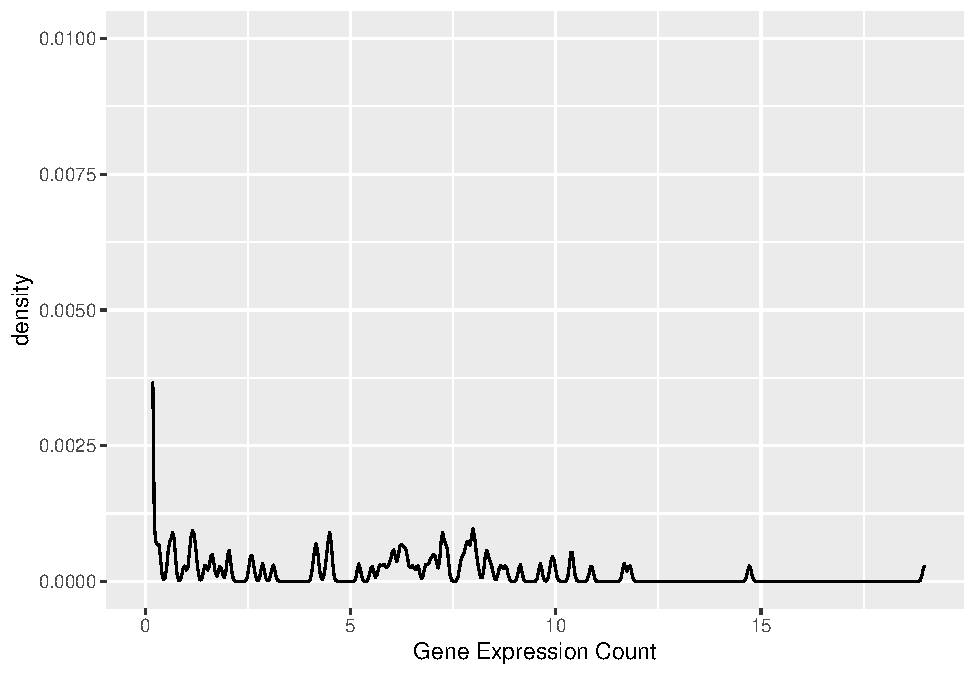
\includegraphics{Assignment2_luft_files/figure-latex/unnamed-chunk-3-1.pdf}
The density plot shows a left skewed distribution of gene expression
counts with most of the expressions being between 0 and 10 but with a
few outliers between 10 and 15. We downloaded the un-normalized data,
however when we opened the raw file, most count values were 0 or very
close to 0. We suspect the data came pre-normalized, and this is causing
some issues. This carries over through the entire assignment.

\subsection{Task 2 - Principal Component
Analysis}\label{task-2---principal-component-analysis}

We were able to get a PCA, tsne, and umap plot following the tutorials.
All three show a clear difference between the healthy control (hs) and
MS (ms) groups, with a few samples in the midst of the other cluster.
The number of crossovers is different.

\subsubsection{PCA Plot}\label{pca-plot}

\begin{figure}
\centering
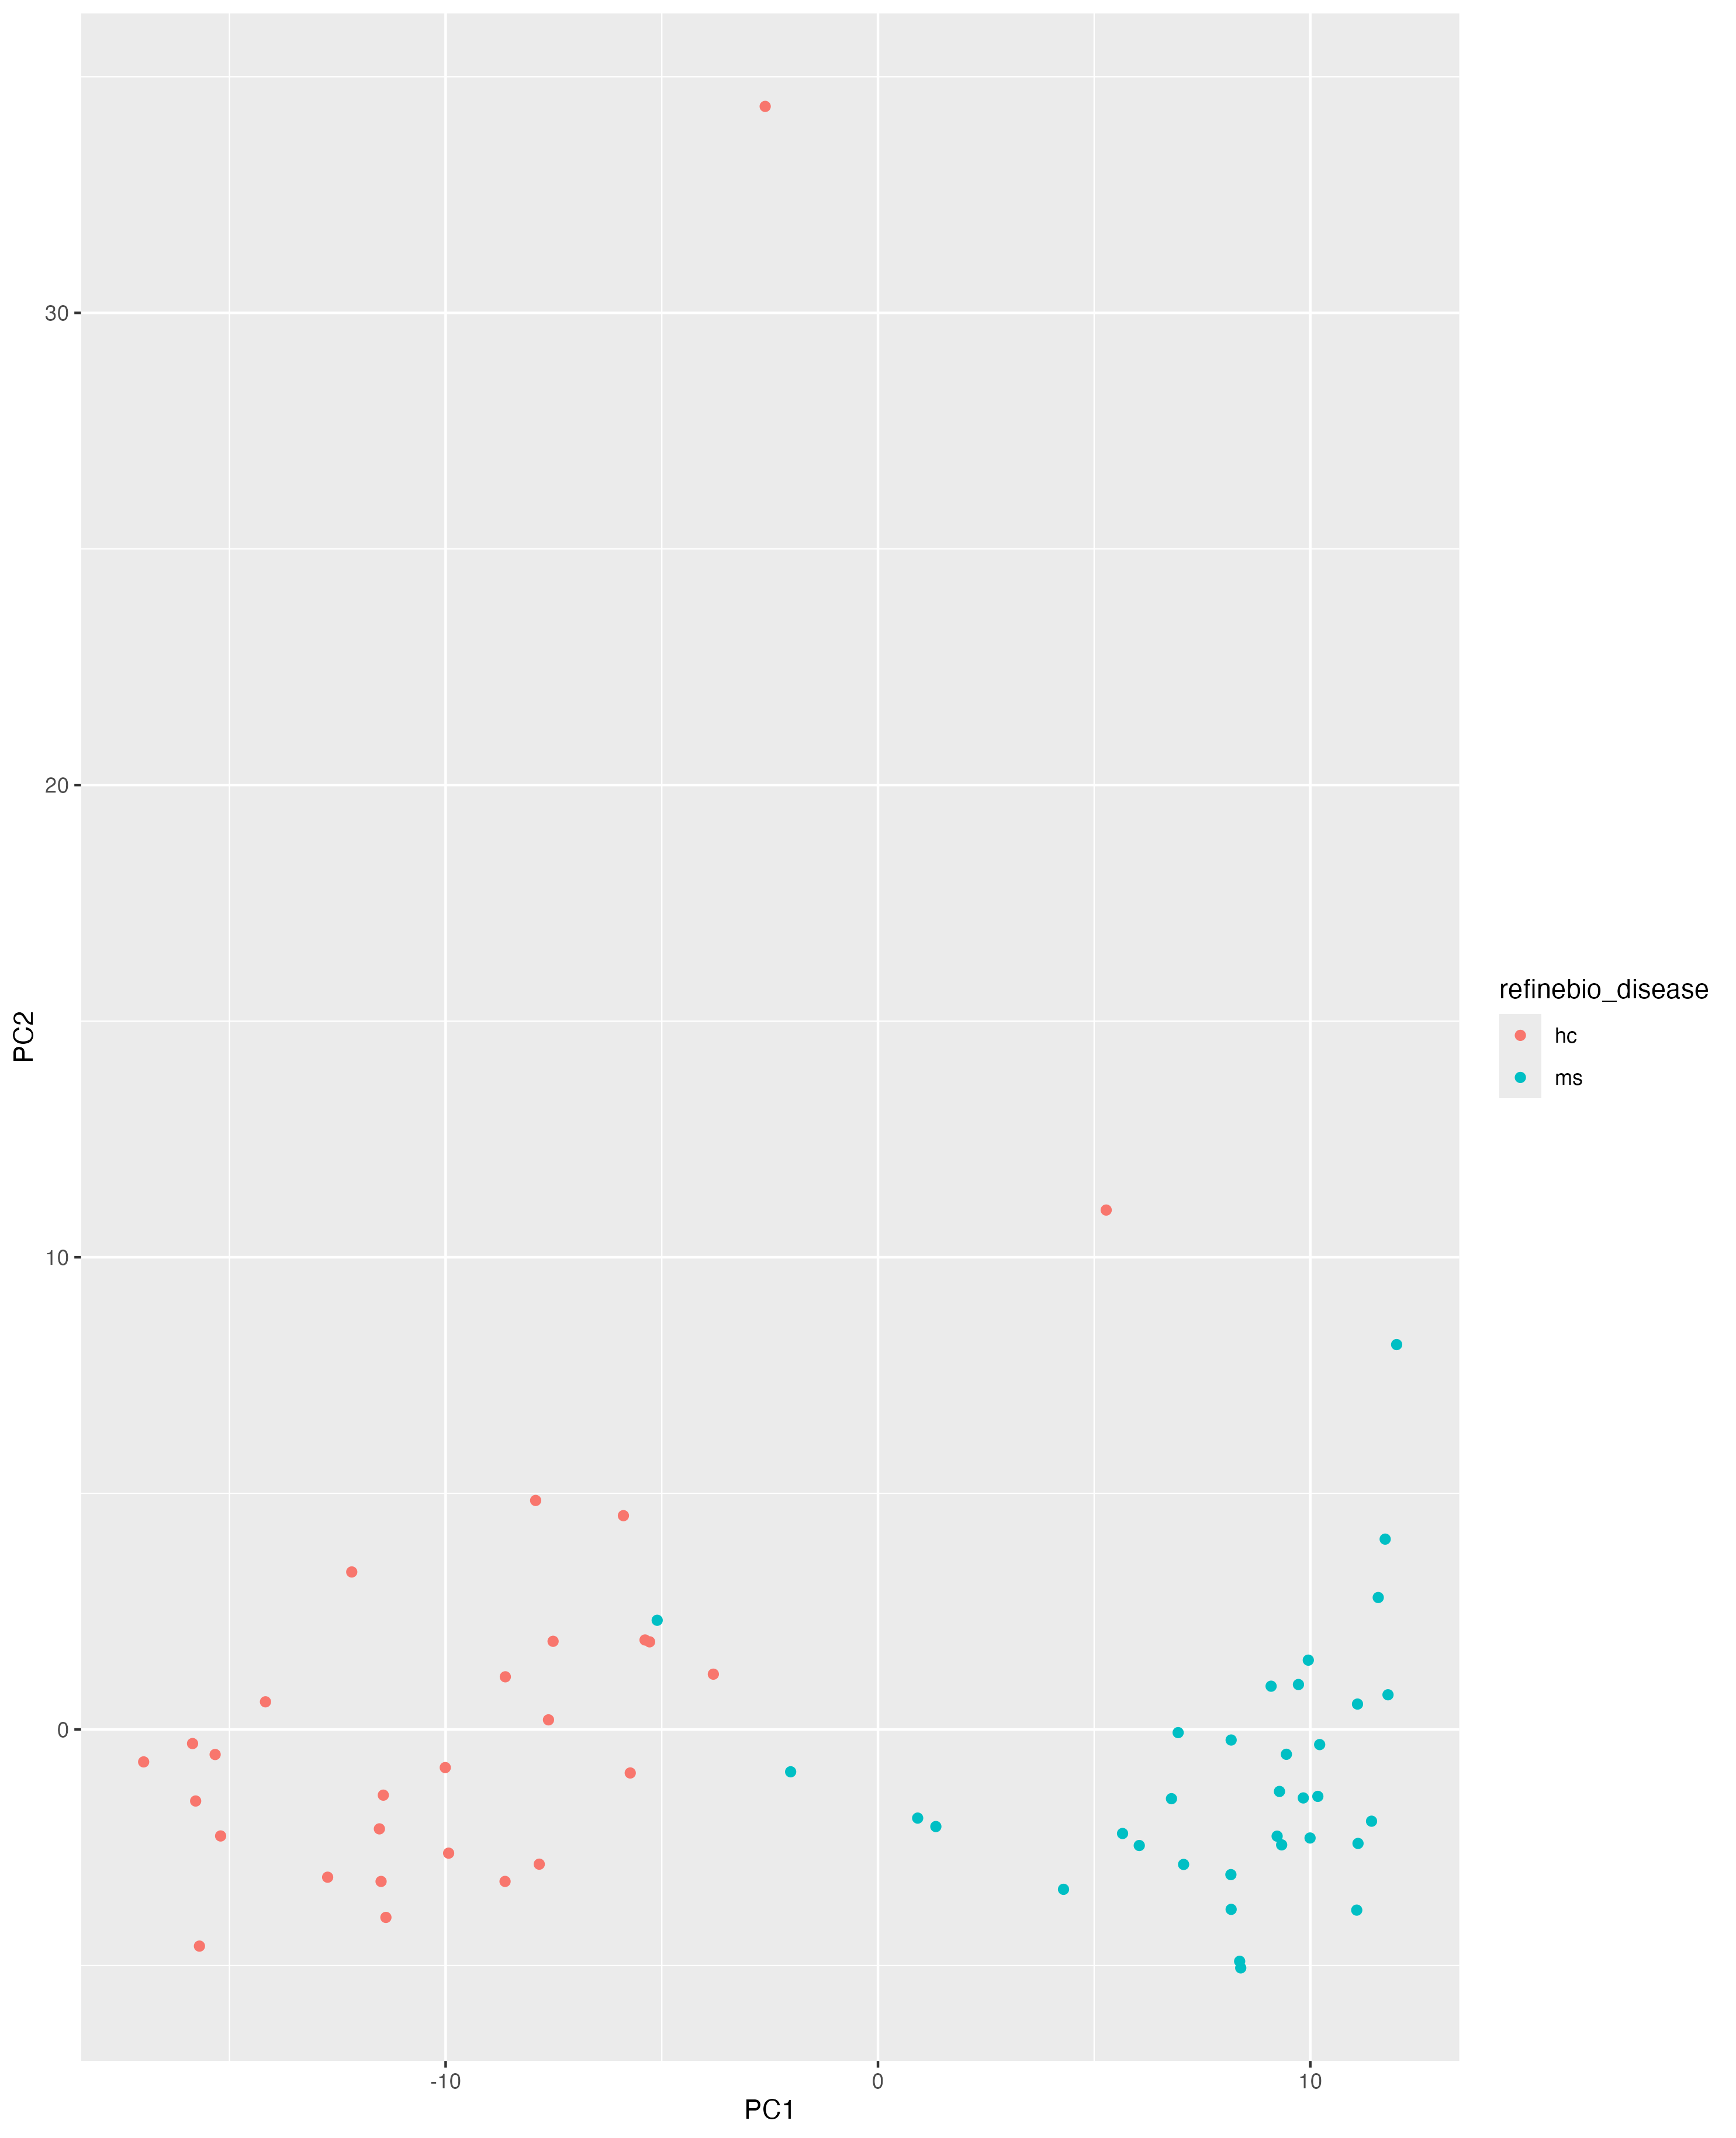
\includegraphics{../../plots/SRP164913_pca_plot.png}
\caption{PCA Plot}
\end{figure}

\newpage

\subsubsection{TSNE Plot}\label{tsne-plot}

\begin{figure}
\centering
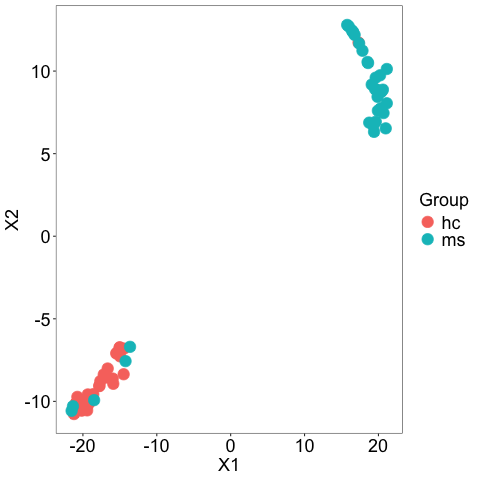
\includegraphics{../../plots/SRP164913_tsne_plot.png}
\caption{tsne Plot}
\end{figure}

\newpage

\subsubsection{UMAP Plot}\label{umap-plot}

\begin{figure}
\centering
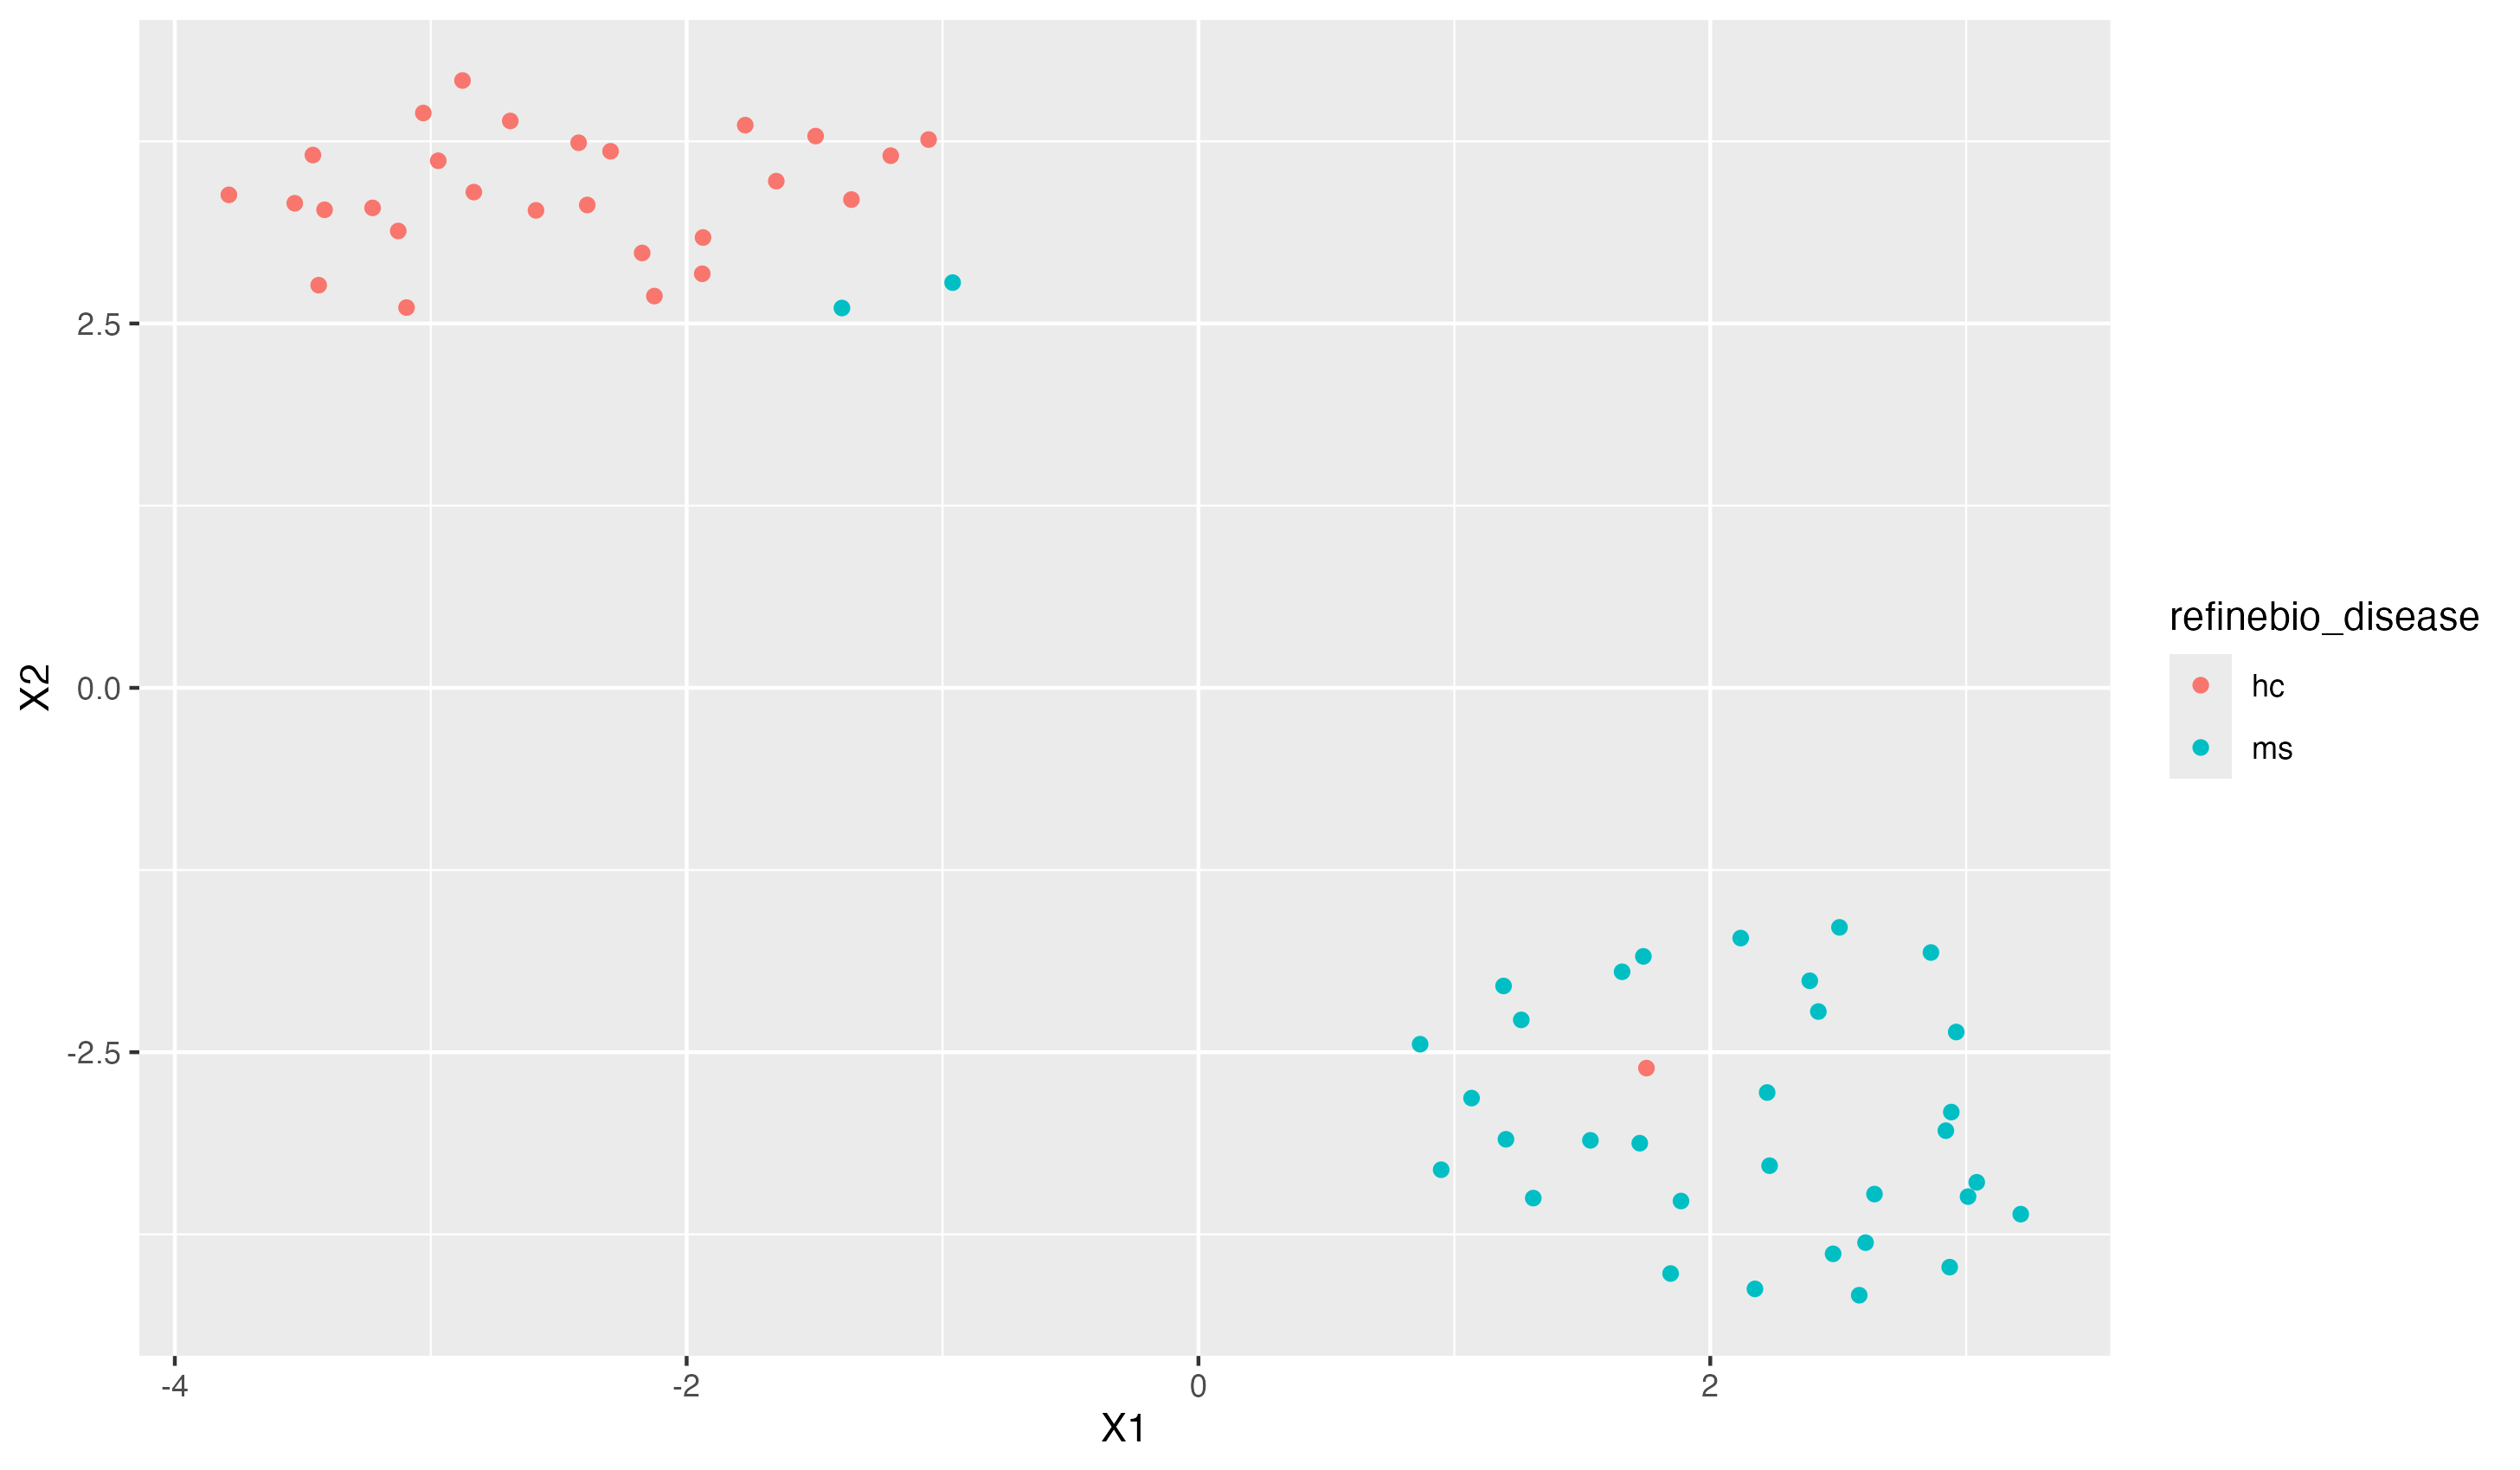
\includegraphics{../../plots/SRP164913_umap_plot.png}
\caption{umap Plot}
\end{figure}

\subsection{Task 3 - Differential
Analysis}\label{task-3---differential-analysis}

When we did our differential analysis, because the data was so small and
normalized, we had to adjust the filter value to 0.01 or else only
\textasciitilde1000 rows were making it to the DESeqDataSetFromMatrix()
step. This was causing our volcano plot to look very sparse. We were
able to get a list of the top 50 differentially expressed genes. The
results, both the entire table and only the top 50, are stored in the
results folder.

\begin{Shaded}
\begin{Highlighting}[]
\NormalTok{top\_50\_file }\OtherTok{\textless{}{-}} \FunctionTok{file.path}\NormalTok{(results\_dir, }\StringTok{"SRP164913\_diff\_expr\_top\_50\_results.tsv"}\NormalTok{)}
\NormalTok{top\_50 }\OtherTok{\textless{}{-}}\NormalTok{ readr}\SpecialCharTok{::}\FunctionTok{read\_tsv}\NormalTok{(top\_50\_file)}
\end{Highlighting}
\end{Shaded}

\begin{verbatim}
## Rows: 50 Columns: 7
## -- Column specification --------------------------------------------------------
## Delimiter: "\t"
## chr (1): Gene
## dbl (5): baseMean, log2FoldChange, lfcSE, pvalue, padj
## lgl (1): threshold
## 
## i Use `spec()` to retrieve the full column specification for this data.
## i Specify the column types or set `show_col_types = FALSE` to quiet this message.
\end{verbatim}

\begin{Shaded}
\begin{Highlighting}[]
\FunctionTok{head}\NormalTok{(top\_50)}
\end{Highlighting}
\end{Shaded}

\begin{verbatim}
## # A tibble: 6 x 7
##   Gene     baseMean log2FoldChange lfcSE        pvalue        padj threshold
##   <chr>       <dbl>          <dbl> <dbl>         <dbl>       <dbl> <lgl>    
## 1 TRBV23-1     9.45          2.34  0.614 0.000168      0.00652     TRUE     
## 2 TRBV16      18.9           1.63  0.424 0.0633        0.0663      FALSE    
## 3 TRBV7-7    557.            1.39  0.269 0.0000000137  0.00000158  TRUE     
## 4 TRBV7-4     31.7           1.15  0.362 0.000108      0.00435     TRUE     
## 5 TRBV12-4   389.            1.02  0.509 0.000837      0.0234      TRUE     
## 6 TRBV15     729.            0.936 0.172 0.00000000247 0.000000326 TRUE
\end{verbatim}

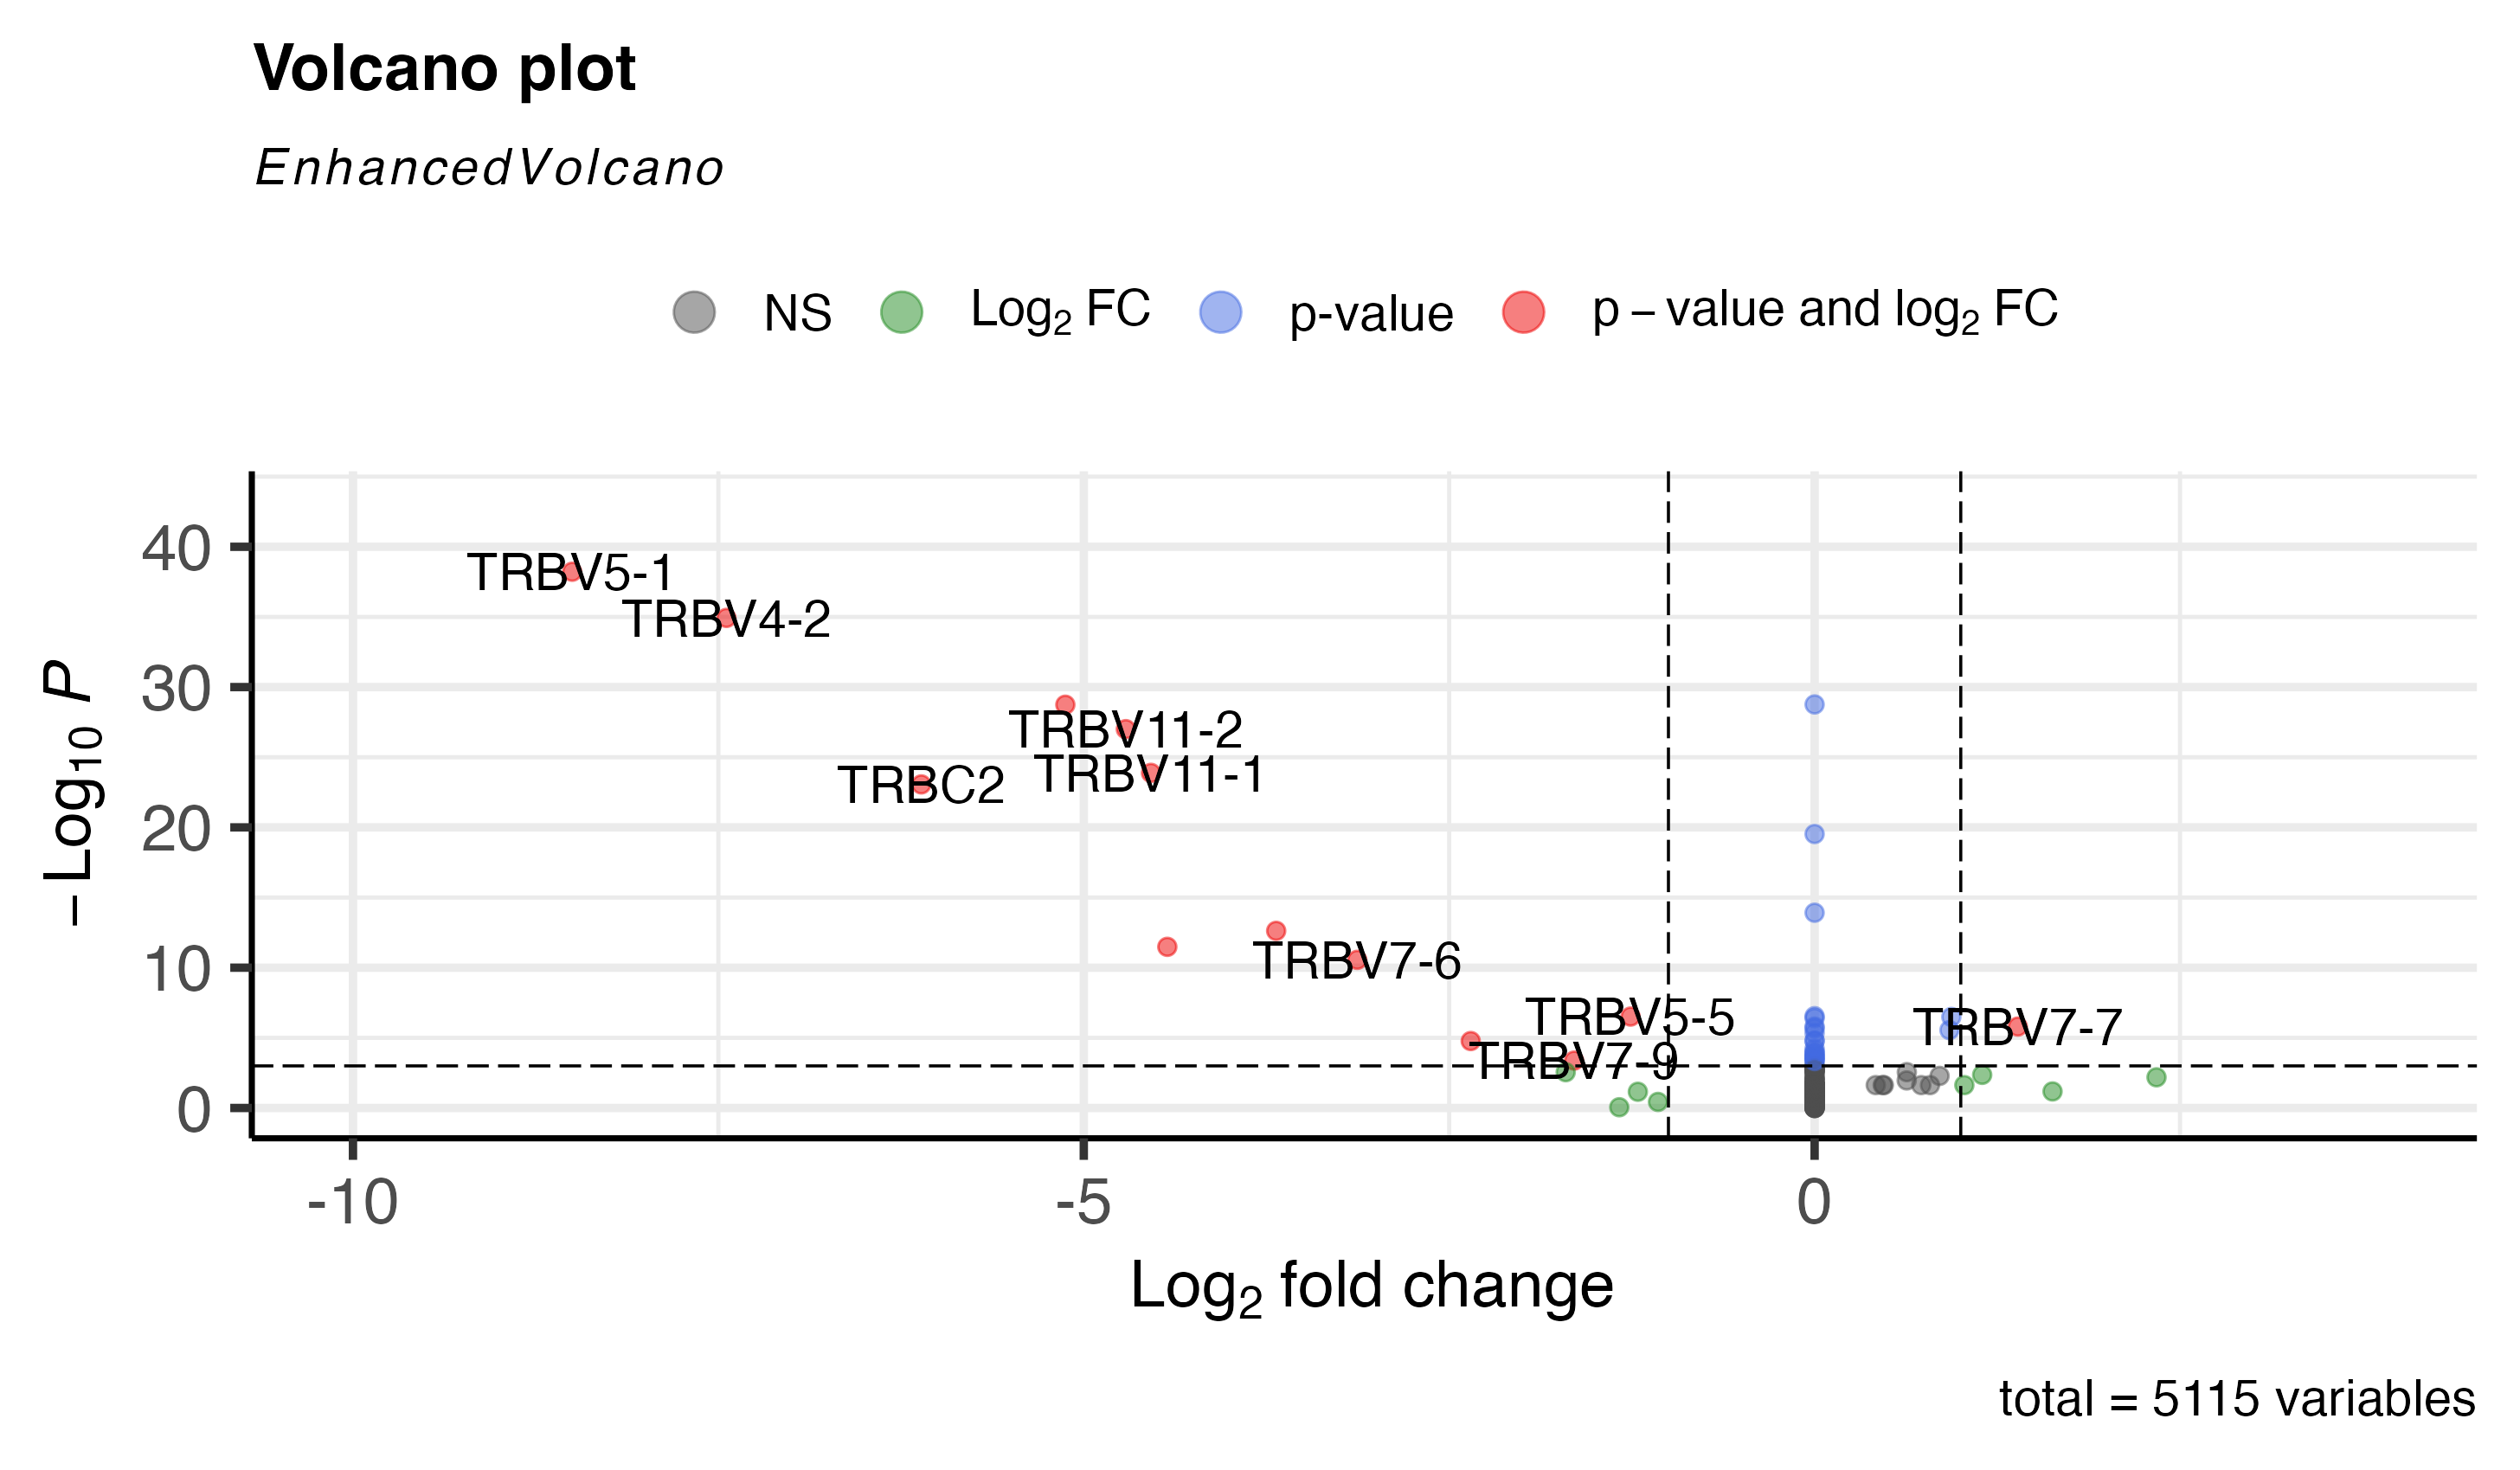
\includegraphics{../../plots/SRP164913_volcano_plot.png} The volcano
plot, while still somewhat sparse, is far more populated than it was
with the highly filtered data. Most significant results have a negative
log fold change.

\newpage

\subsection{Task 4 - Heatmap}\label{task-4---heatmap}

A heatmap was generated for the top 50 differentially expressed genes.
The counts for each gene in the top 50 were extracted and put into the
heatmap plot. It was annotated with the two disease groups: ms subjects
and healthy control subjects. Since many of our counts are 0 and
therefore are not expressed differently, the map is largely blue.

\begin{figure}
\centering
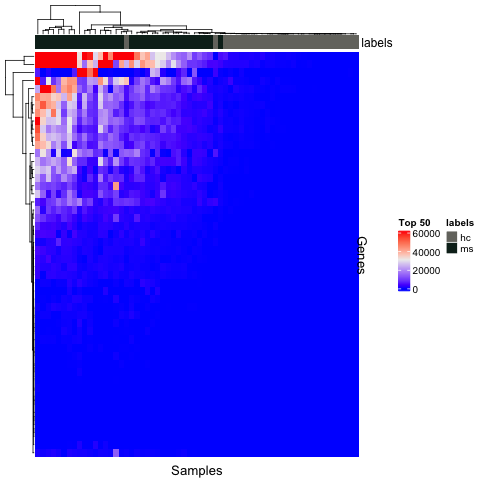
\includegraphics{../../plots/SRP164913_heatmap_plot.png}
\caption{Heatmap}
\end{figure}

\subsection{Task 5 - Enrichment
Analysis}\label{task-5---enrichment-analysis}

\subsubsection{Hannah- gprofiler2}\label{hannah--gprofiler2}

The function gost was used from gprofiler2 to perform enrichment
analysis on the differentially expressed data. Disease ontology was
used, as the data was differentially expressed between the MS subjects
and healthy controls. Only genes with adjusted p-values below 0.05 were
put into the function. Two gost results were generated: one that
contains all results, significant or not, and one that contained only
significant results. The plot (created with gostplot) for the
significant results is shown below. It seems there are a few points
above the significance threshold.

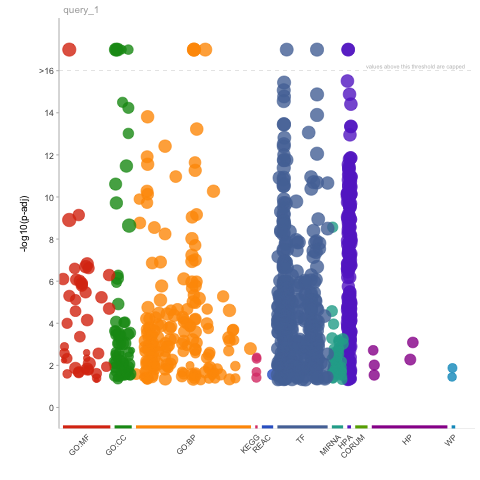
\includegraphics{../../plots/SRP164913_gprofiler_gostplot.png} However,
when publish\_gosttable(gost\_res3) was run, the function would not
complete. It would continue to run for over 15 minutes and never produce
results. I was unable to generate a table from the results, and when I
tried to print the results, it would return NULL for both significant
and non-significant gost results. The NULL result is shown below along
with the gost function that was run. It is possible that no truly
significant results were generated and so the results were empty.

\begin{Shaded}
\begin{Highlighting}[]
\NormalTok{results\_dir }\OtherTok{\textless{}{-}} \FunctionTok{file.path}\NormalTok{(}\StringTok{"../../results"}\NormalTok{)}
\NormalTok{diff\_expr\_file }\OtherTok{\textless{}{-}} \FunctionTok{file.path}\NormalTok{(results\_dir, }\StringTok{"SRP164913\_diff\_expr\_results.tsv"}\NormalTok{)}
\FunctionTok{library}\NormalTok{(gprofiler2)}
\NormalTok{diff\_expr\_df }\OtherTok{\textless{}{-}}\NormalTok{ readr}\SpecialCharTok{::}\FunctionTok{read\_tsv}\NormalTok{(diff\_expr\_file)}
\end{Highlighting}
\end{Shaded}

\begin{verbatim}
## Rows: 5115 Columns: 7
## -- Column specification --------------------------------------------------------
## Delimiter: "\t"
## chr (1): Gene
## dbl (5): baseMean, log2FoldChange, lfcSE, pvalue, padj
## lgl (1): threshold
## 
## i Use `spec()` to retrieve the full column specification for this data.
## i Specify the column types or set `show_col_types = FALSE` to quiet this message.
\end{verbatim}

\begin{Shaded}
\begin{Highlighting}[]
\NormalTok{gost\_res3 }\OtherTok{\textless{}{-}} \FunctionTok{gost}\NormalTok{(}
  \AttributeTok{query =} \FunctionTok{unlist}\NormalTok{(diff\_expr\_df[diff\_expr\_df}\SpecialCharTok{$}\NormalTok{padj}\SpecialCharTok{\textless{}}\FloatTok{0.05}\NormalTok{, }\StringTok{\textquotesingle{}Gene\textquotesingle{}}\NormalTok{]), }
  \AttributeTok{significant=}\ConstantTok{TRUE}\NormalTok{, }
  \AttributeTok{organism =} \StringTok{"hsapiens"}
\NormalTok{  ) }
\FunctionTok{head}\NormalTok{(gost\_res3}\SpecialCharTok{$}\NormalTok{results)}
\end{Highlighting}
\end{Shaded}

\begin{verbatim}
## NULL
\end{verbatim}

When I had initially tried to run gost with every gene name, no p-value
factor, it would produce a result that could be printed, but that is not
as relevant to our dataset. This does prove that something is off with
specifically the differential data, and the function does work.

Unfortunatly, due to the circumstances described above, no table was
generated using the gprofiler2 method.

\subsubsection{Luca - topGO}\label{luca---topgo}

Given a set of genes and a gene differential expression analysis, topGo
enriches the most relevant Genes with Gene Ontology (GO) terms. This
helps to find out what function the differential expressed genes perform
in the Human Body.

\paragraph{Methodology}\label{methodology}

The Mothodology described is analogous to the Quick Start Guide found
here
``\url{https://bioconductor.org/packages/release/bioc/vignettes/topGO/inst/doc/topGO.pdf}''.
The Output of Task 1-4 was a list of differential expressed genes, with
their probability, only trivial transformations were required to input
the data into the topGO function which returns an object containing all
gene identifiers and their scores, GO annotations and further
information. The cutoff for expressed gene selection has been set to the
default of p\textless0.05.

Using the Fisher exact test a enrichment analysis is performed, testing
for the over-representation of GO terms within the differentially
expressed genes. Due to time constraints only the classic method,
testing each GO category independently was used.

\paragraph{Results:}\label{results}

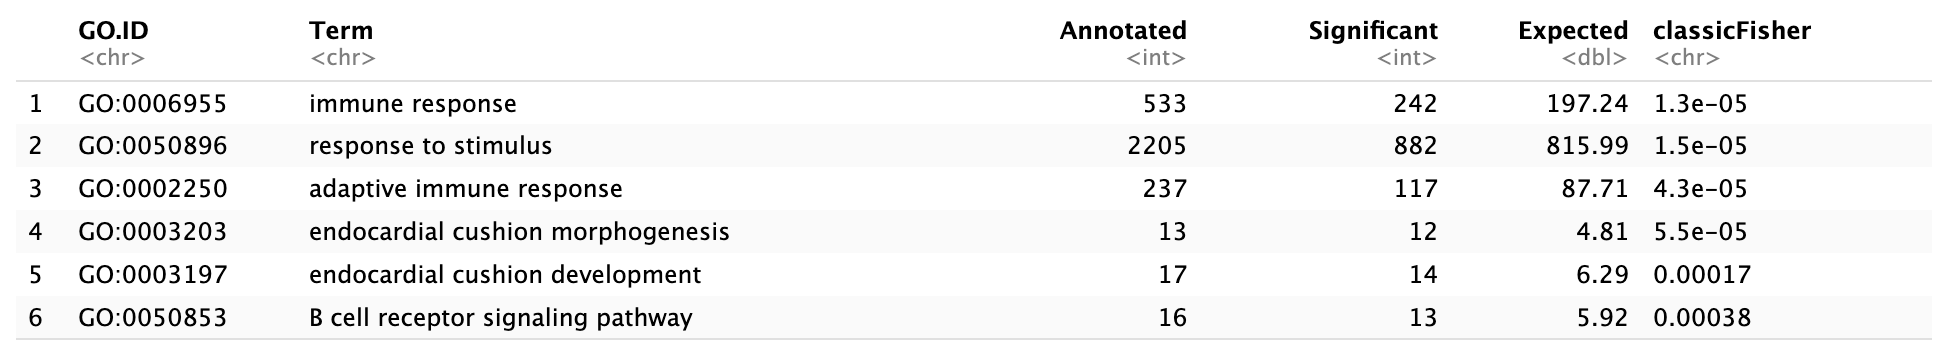
\includegraphics{../../plots/SRP164913_topGO_top_6.png} The Table above,
shows the first few rows of the enrichment analysis. Although the issues
with the pre-normalized data mentioned in the introduction, parts of the
result seem plausible to the untrained eye in regard to the disease
Multiple Sclerosis (This is the first time I actually experienced joy
during this assignment). In multiple sclerosis MS, the immune system
attacks the protective cover on nerve, causing communication problems
between the brain and the rest of the body. Due to this pathology it is
coherent, that the top differential expressed genes found during the
enrichment analysis, are genes and receptors linked to the immune
system. Below the most significant 5 nodes are represented as a tree.
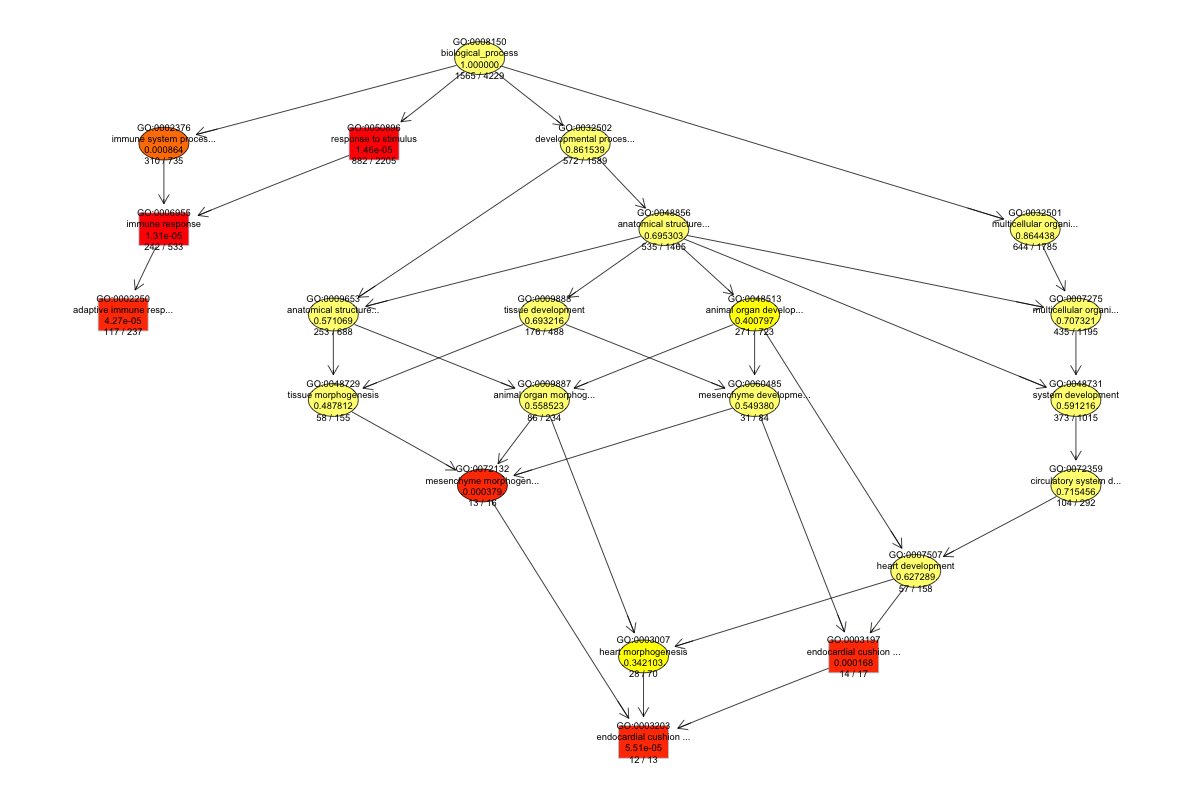
\includegraphics{../../plots/SRP164913_topGO_tree.png}

\paragraph{Fisher vs Elim}\label{fisher-vs-elim}

Due to time constraint, only Fisher's exact test was used to generate
the above results. To visualize the potential differences the following
plot, shows that the Elim test would yield higher p-values for multiple
genes, while some are identical for both methods.

\includegraphics{../../plots/SRP164913_topGO_fisher_vs_elim.png}

\subsection{Task 6/7 - Joint Enrichment
Analysis}\label{task-67---joint-enrichment-analysis}

\end{document}
